\documentclass{beamer}
\usetheme{Darmstadt}
\usepackage{graphicx}
\usepackage{wrapfig}
\usepackage[utf8]{inputenc}
\usepackage{float}
\usepackage{verbatim}
\RequirePackage{etoolbox}
\beamerdefaultoverlayspecification{<+->}
\begin{document}

\title{CS251: Box2d Project Report by Group 10}
\author{\begin{tabular}{ c c c }
				 Krishna & Rohith & Goutham \\ 
	   			140050038 & 140050060 & 140050065 \\ 
				140050038@iitb.ac.in & 140050060@iitb.ac.in & 140050065@iitb.ac.in \\ 
	   		\end{tabular}}
\date{\today}
\begin{frame}
\titlepage
\end{frame}

\section{Outline}
\begin{frame}
\tableofcontents
\subsection{Motivation}
\subsection{Introduction}
\subsection{Design of the simulation}
\subsection{Simulation Steps}
\subsection{Conclusion}
\end{frame}

\begin{frame}{Motivation}
Box2d makes a great general benchmark, its a bottleneck on real-world apps. 
So we took it upon ourselves to put together a little benchmark that shows how hard can one actually perform a task which can be done in a very simple manner i.e; Goldberg Machine.So,We are using this Box2D,a 2-dimensional physics simulation engine (written in C++) to code/implement it.Every night before sleeping we put on our alarm and also will be good enough lazy to turn it off and gets irritated in the morning as it starts buzzing.It happened to me personally when I was in a nice dream and want no one to become victim like me.This laid the foundations of our project.
\end{frame}

\begin{frame}{Introduction}
\begin{itemize}
\item A Rube Goldberg machine is a deliberately over-engineered or overdone machine that performs a very simple task in a very complex fashion, usually including a chain reaction. In this project we have are going to create a simulation of a Rube Goldberg machine we designed, in C++ using the Box2D library

\item The Rube Goldberg machine's final aim is to turn off the buzzing alarm by just pulling the thread.In this Document we have given a gist of our design, its salient features and working
\end{itemize}
\end{frame}

\begin{frame}{Design of the Simulation}
	
	 This is how the simulation looks like and starts with the pendulum
    \begin{center}
     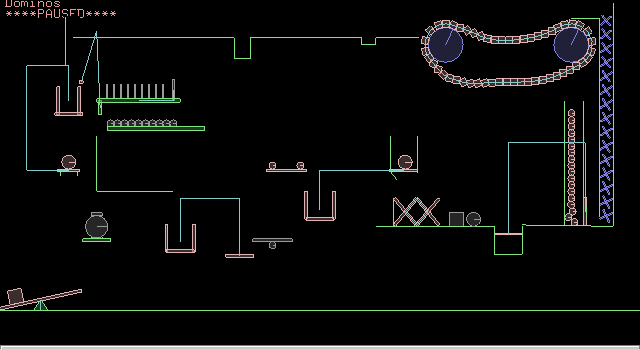
\includegraphics[width=1.0\textwidth]{2.png}
     \end{center}
\end{frame}

\begin{frame}{Simulation Steps}
Simulation starts with pendulum.This hits the series of dominos which inturn hits a series of  spheres.When these spheres fall into the basket kind of object leading to the raise of balloon.This results in the release of a sphere which initiates the expansion of the spring.This releases a heap of balls, which are lifted up and throwed on to a conveyor belt by series of rotating wheels that act as vertical lifters. This finally concludes the process by uplifting the wedge and hence moving the weight on the alarm.
\end{frame}

\begin{frame}{Conclusion}
We hope this presentation has served your purpose and made easier for you to know about the simulation.Thank You !!
\end{frame}



\end{document}
